% VLDB WORKSHOP template version of 2024-05-15 enhances the ACM template, version 1.7.0:
% https://www.acm.org/publications/proceedings-template
% The ACM Latex guide provides further information about the ACM template.

\documentclass[sigconf, nonacm]{acmart}

\newcommand\vldbyear{2026}
\newcommand\vldbworkshop{Quality in Databases (QDB)}
\newcommand\vldbauthors{\authors}
\newcommand\vldbtitle{\shorttitle}
\newcommand\vldbavailabilityurl{}
\newcommand\vldbpagestyle{plain}

\begin{document}

\title[Medici\'on de credibilidad en redes sociales]{Medici\'on de credibilidad en plataformas de redes sociales mediante calidad de datos y provenance}

\author{Sebasti\'an Garc\'ia Parra}
\affiliation{%
  \institution{Facultad de Ingenier\'ia, Universidad de la Rep\'ublica}
  \city{Montevideo}
  \country{Uruguay}
}
\email{dgparra@fing.edu.uy}

\author{Adriana Marotta}
\affiliation{%
  \institution{Facultad de Ingenier\'ia, Universidad de la Rep\'ublica}
  \city{Montevideo}
  \country{Uruguay}
}
\email{amarotta@fing.edu.uy}

\begin{abstract}
Las plataformas de redes sociales se han convertido en fuentes primarias de
informaci\'on para decisiones de salud, pol\'itica, crisis y vida cotidiana. Sin
embargo, los usuarios suelen consumir y propagar contenido sin indicadores
objetivos sobre su credibilidad, especialmente cuando una publicaci\'on es copiada,
modificada o compartida entre plataformas. Este paper presenta un modelo de
calidad de datos para medir la credibilidad de clips en redes sociales. El modelo
organiza la credibilidad en dos dimensiones principales: trustworthiness, calculada
a partir de reputation, verifiability y expertise, y provenance, que captura el
origen y la evoluci\'on de un clip. Se introduce Trustworthiness Path Stability,
una m\'etrica de calidad que eval\'ua si el trustworthiness permanece estable a lo
largo del provenance. Tambi\'en se describe un flujo modular que normaliza clips
heterog\'eneos, genera features de dominio, calcula m\'etricas de calidad y
reconstruye provenance mediante interacciones expl\'icitas y equivalencia textual.
Una prueba de concepto sobre publicaciones acerca de estatinas y colesterol,
validada con un experto m\'edico, muestra alta concordancia entre el modelo y la
evaluaci\'on experta.
\end{abstract}

\maketitle

%%% do not modify the following VLDB block %%
%%% VLDB block start %%%
\pagestyle{\vldbpagestyle}
\begingroup\small\noindent\raggedright\textbf{VLDB Workshop Reference Format:}\\
\vldbauthors. \vldbtitle. VLDB \vldbyear\ Workshop: \vldbworkshop.\\
\endgroup
\begingroup
\renewcommand\thefootnote{}\footnote{\noindent
This work is licensed under the Creative Commons BY-NC-ND 4.0 International License. Visit \url{https://creativecommons.org/licenses/by-nc-nd/4.0/} to view a copy of this license. For any use beyond those covered by this license, obtain permission by emailing \href{mailto:info@vldb.org}{info@vldb.org}. Copyright is held by the owner/author(s). Publication rights licensed to the VLDB Endowment. \\
\raggedright Proceedings of the VLDB Endowment.
ISSN 2150-8097. \\
}\addtocounter{footnote}{-1}\endgroup
%%% VLDB block end %%%

%%% do not modify the following VLDB block %%
%%% VLDB block start %%%
\ifdefempty{\vldbavailabilityurl}{}{
\vspace{.3cm}
\begingroup\small\noindent\raggedright\textbf{VLDB Workshop Artifact Availability:}\\
The source code, data, and/or other artifacts have been made available at \url{\vldbavailabilityurl}.
\endgroup
}
%%% VLDB block end %%%

\section{Introducci\'on}

El contenido producido en redes sociales se utiliza cada vez m\'as como evidencia
para decisiones con consecuencias online y offline. Un usuario puede decidir si
comparte una publicaci\'on, conf\'ia en una fuente, acepta un consejo m\'edico o
rechaza un tratamiento a partir de informaci\'on cuya calidad es incierta. Este
riesgo aumenta por la velocidad con que las plataformas promueven la difusi\'on y
por la ausencia de est\'andares para preservar metadatos de calidad cuando el
contenido cruza fronteras entre plataformas.

Los mecanismos actuales, como cuentas verificadas o anotaciones comunitarias,
aportan se\~nales \'utiles pero no ofrecen una visi\'on general de calidad de datos
sobre la credibilidad. Adem\'as, los usuarios participan en varias plataformas y el
contenido puede ser copiado manualmente, citado, parafraseado o republicado sin
conservar los metadatos de la fuente original. As\'i, una misma pieza de
informaci\'on puede aparecer en varias versiones, con distintos autores, evidencias,
audiencias y contextos de confianza.

Este problema no es solo detecci\'on de desinformaci\'on. Muchos enfoques clasifican
un post, un tema o una fuente como cre\'ible o no cre\'ible, pero ocultan las razones
del score. Desde calidad de datos, esto es insuficiente: un consumidor, periodista
o experto de dominio necesita saber si un valor bajo proviene de falta de evidencia,
escasa expertise de la fuente, baja reputation o un camino de propagaci\'on inestable.
El objetivo de este trabajo es que la credibilidad sea medible, descomponible y
auditable.

Este paper condensa una tesis de maestr\'ia sobre medici\'on de credibilidad en
plataformas de redes sociales~\cite{GarciaParra2024Thesis}. Su contribuci\'on principal es un modelo de calidad
de datos, sensible al provenance, para evaluar clips. Un clip representa una unidad
de informaci\'on social: post, tweet, comentario, caption de video o publicaci\'on
espec\'ifica de una plataforma. El modelo es agn\'ostico de la red social y adaptable
al dominio: un experto en calidad de datos define dimensiones y m\'etricas, mientras
que un experto de dominio ajusta ponderadores y umbrales.

El trabajo realiza tres contribuciones. Primero, define un modelo de calidad para
credibilidad que combina trustworthiness y provenance. Segundo, introduce
Trustworthiness Path Stability, una m\'etrica para capturar c\'omo cambia la
confianza cuando el contenido se propaga y transforma. Tercero, presenta un flujo
modular de procesamiento y una prueba de concepto en el dominio m\'edico, enfocada
en contenido sobre estatinas y colesterol.

\section{Antecedentes y Requisitos}

La credibilidad ha sido tratada como una calidad percibida y no como una propiedad
inherente de un objeto~\cite{FoggTseng1999}. Desde la calidad de datos, la
credibilidad se relaciona con trustworthiness, reputation y provenance
~\cite{BatiniScannapieco2016}. En redes sociales esta relaci\'on es especialmente
importante porque la evaluaci\'on ocurre bajo incertidumbre: el usuario ve solo una
parte del contexto original, y la autoridad aparente de una fuente puede resultar
enga\~nosa.

Trabajos sobre credibilidad en Twitter/X muestran que caracter\'isticas del mensaje,
del usuario, del tema y de la propagaci\'on ayudan a estimar credibilidad
~\cite{Castillo2011}. Otros trabajos abordan la calidad de datos en redes sociales
y adaptan dimensiones tradicionales de calidad a flujos de tweets
~\cite{Arolfo2020}. Estudios recientes muestran adem\'as que la expertise de la
fuente y las creencias previas influyen fuertemente en la evaluaci\'on de
publicaciones, en particular en dominios de salud~\cite{Kuutila2024}.

El provenance ofrece una mirada complementaria. El linaje de datos captura origen,
derivaci\'on y transformaciones, y ha sido reconocido como mecanismo central para
evaluar confianza en productos de datos~\cite{Simmhan2005}. PROV-SAID extiende
W3C PROV para representar difusi\'on de informaci\'on en redes sociales
~\cite{Taxidou2015}. Modela mensajes, agentes, influencia e interacciones, pero su
formulaci\'on original no modela directamente el cross-sharing ni m\'etricas de
calidad asociadas al camino de provenance.

De estas observaciones se derivan cuatro requisitos. El modelo debe ser agn\'ostico
de plataforma, porque las se\~nales var\'ian entre X, Facebook, TikTok, Reddit,
WhatsApp y otras redes. Debe ser sensible al provenance, porque la credibilidad
puede cambiar cuando el contenido se copia, revisa o comparte. Debe admitir
m\'etricas espec\'ificas de dominio, porque medicina, pol\'itica y emergencias
requieren evidencias distintas. Finalmente, debe ser modular para incorporar nuevos
generadores de features, m\'etricas y estrategias de b\'usqueda.

Un requisito adicional es la interpretabilidad. El modelo est\'a pensado para varios
roles: usuarios finales que consumen indicadores de credibilidad, expertos en calidad
de datos que configuran m\'etricas y expertos de dominio que validan ponderadores,
umbrales y ejemplos. Por esa raz\'on, el modelo evita tratar la credibilidad como una
etiqueta opaca y expone las dimensiones que contribuyen al resultado final.

\section{Modelo de Calidad}

Modelamos \emph{Credibility} como un cluster compuesto por dos dimensiones:
\emph{Trustworthiness} y \emph{Provenance}. Trustworthiness estima la confiabilidad
esperada del clip dentro de su dominio. Provenance captura origen, derivaci\'on y
propagaci\'on.

\begin{figure*}[t]
  \centering
  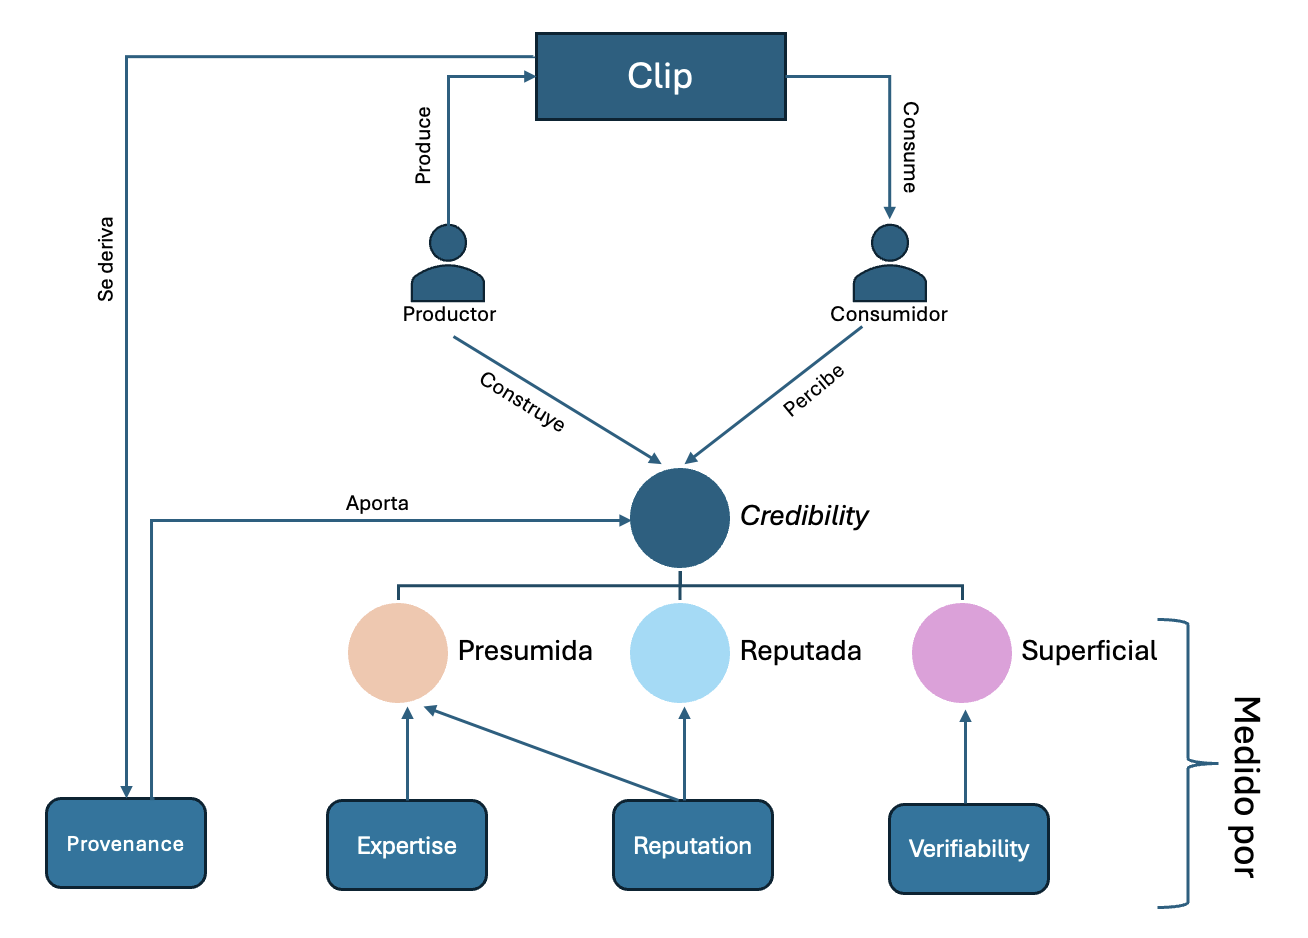
\includegraphics[width=.82\textwidth,height=.42\textheight,keepaspectratio]{figures/credibility-dq-composition}
  \caption{Composici\'on conceptual de la credibilidad y sus dimensiones de calidad asociadas~\cite{GarciaParra2024Thesis}.}
  \Description{Diagrama con productor, consumidor, clip, credibilidad percibida y los factores de calidad expertise, reputation, verifiability y provenance.}
  \label{fig:credibility-composition}
\end{figure*}

\begin{figure*}[t]
  \centering
  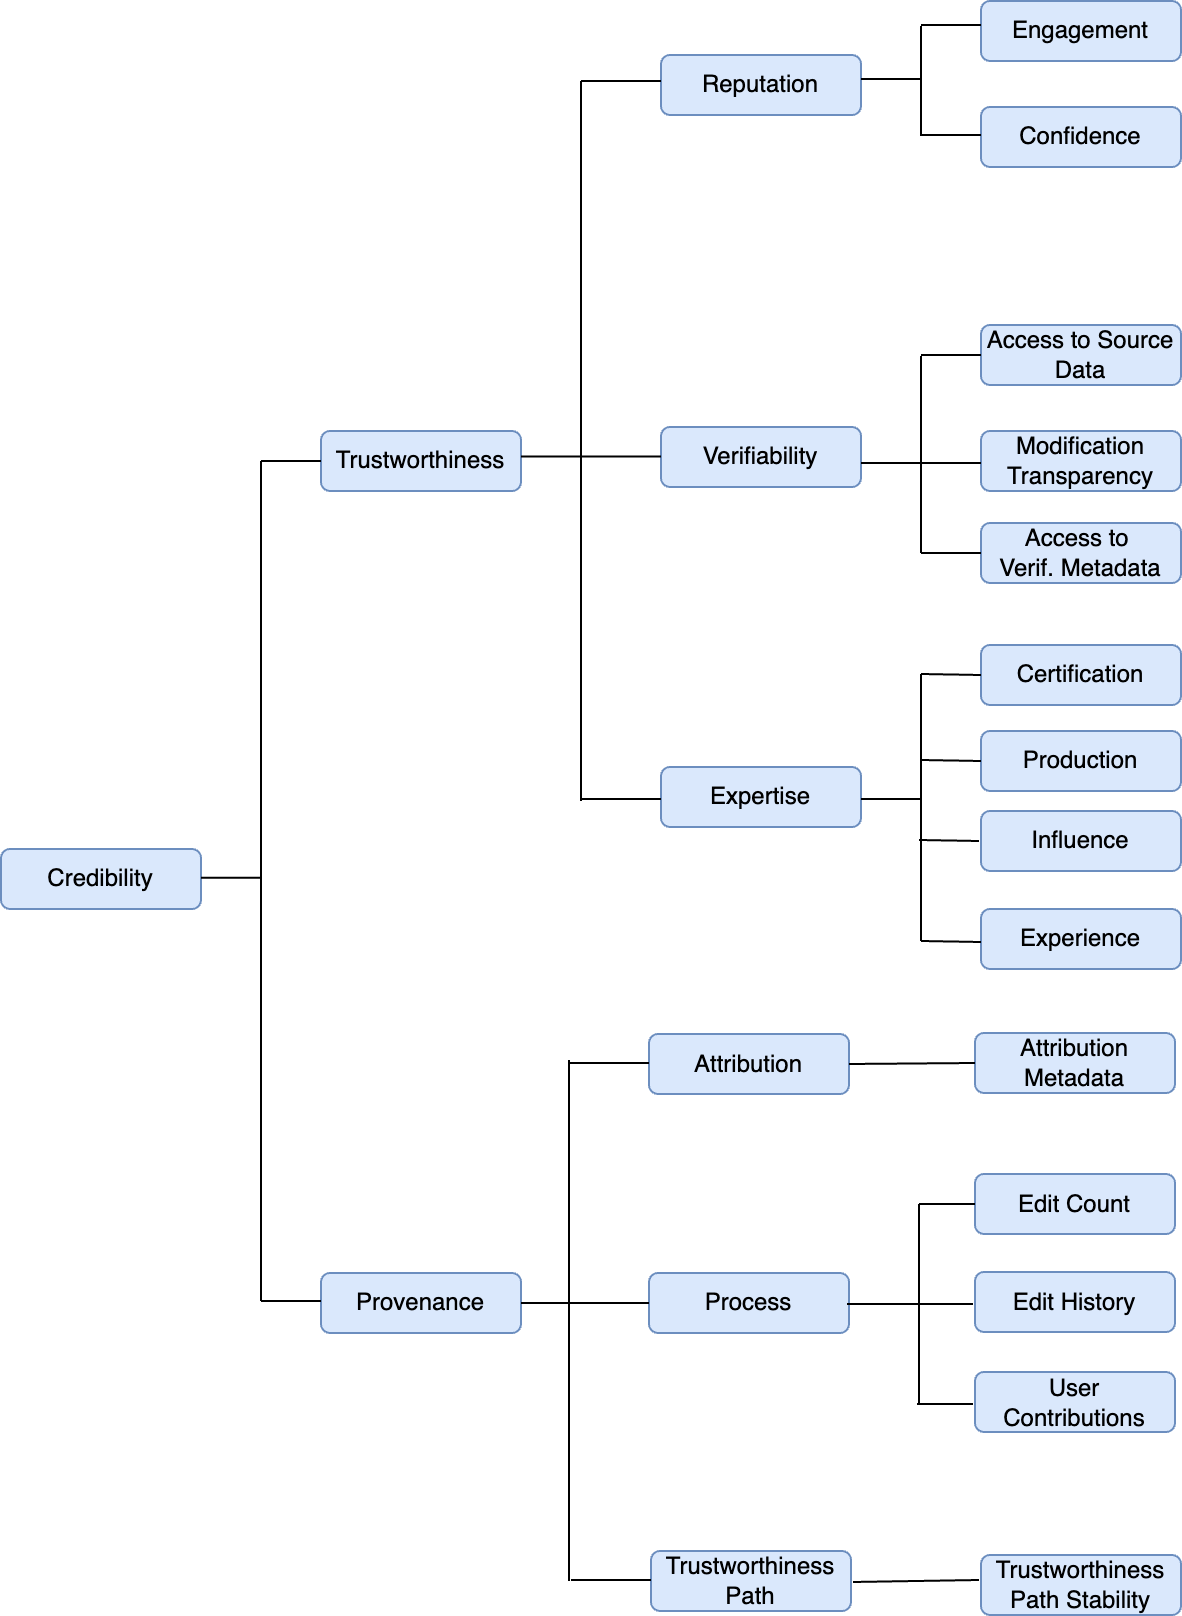
\includegraphics[width=.82\textwidth,height=.70\textheight,keepaspectratio]{figures/credibility-cluster-white}
  \caption{Cluster de calidad para credibilidad~\cite{GarciaParra2024Thesis}.}
  \Description{Jerarqu\'ia de credibilidad, trustworthiness, provenance y sus factores y m\'etricas de calidad.}
  \label{fig:credibility-cluster}
\end{figure*}

Trustworthiness se descompone en tres factores. \emph{Reputation} eval\'ua la
percepci\'on externa del autor o fuente mediante m\'etricas como engagement y
confidence. \emph{Verifiability} eval\'ua si el clip aporta evidencia suficiente para
corroborar sus afirmaciones, incluyendo datos fuente, transparencia de
modificaciones y metadatos de verificaci\'on. \emph{Expertise} eval\'ua si el autor
tiene conocimiento espec\'ifico del dominio, usando m\'etricas como certification,
production, influence y experience.

La necesidad de esta descomposici\'on surge de la forma en que los usuarios juzgan
credibilidad en redes sociales. Como resume \autoref{fig:credibility-composition},
la credibilidad es construida por el productor y percibida por el consumidor, y se
ve afectada por tres facetas definidas por Fogg y Tseng: credibilidad presumida,
reputada y superficial~\cite{FoggTseng1999}. La credibilidad presumida surge de creencias previas y supuestos
culturales, por ejemplo asumir que una persona que parece m\'edica es confiable en
una discusi\'on de salud. La credibilidad reputada surge de evaluaciones de terceros,
avales e historia de la fuente. La credibilidad superficial surge de se\~nales
visibles como una presentaci\'on cuidada, un perfil que parece verificado o un enlace
con apariencia profesional.

Estas facetas son \'utiles, pero tambi\'en son modos de falla. En redes sociales, la
credibilidad presumida puede amplificar sesgos de confirmaci\'on: los usuarios
tienden a creer contenido que coincide con sus creencias incluso cuando la evidencia
es d\'ebil. La credibilidad reputada puede sobrevalorar popularidad, porque una gran
audiencia o muchas interacciones no implican competencia en el dominio. La
credibilidad superficial puede premiar publicaciones que parecen autorizadas aunque
no incluyan datos fuente ni afirmaciones verificables. Por eso, un modelo de calidad
debe exponer expertise, reputation y verifiability por separado. Esta separaci\'on
ayuda a reducir errores de credulidad, donde se acepta contenido de baja calidad
como cre\'ible, y errores de incredulidad, donde se rechaza contenido cre\'ible porque
las se\~nales de calidad relevantes no est\'an visibles.

Provenance se descompone en attribution, process y trustworthiness path.
Attribution identifica fuentes o entidades autoras. Process captura c\'omo se gener\'o
o modific\'o el clip. Trustworthiness path captura c\'omo evoluciona la confianza a lo
largo del camino de provenance.

Provenance es necesario porque la credibilidad en redes sociales no queda fija en el
momento de publicaci\'on. Un clip puede originarse en una instituci\'on confiable,
ser copiado por una cuenta poco confiable, ser parafraseado en otra plataforma y
luego ser compartido por un experto del dominio. A la inversa, una afirmaci\'on
enga\~nosa puede ganar apariencia de credibilidad al pasar por intermediarios
visualmente cre\'ibles o populares. Sin provenance, el modelo solo eval\'ua la
apariencia actual del clip; con provenance, puede preguntar si el clip preserva la
calidad de su fuente, si fue modificado y si el trustworthiness del camino de
propagaci\'on es estable.

\autoref{fig:credibility-cluster} muestra la jerarqu\'ia completa. La decisi\'on de
dise\~no relevante es que provenance no se trata solamente como metadatos para
trazabilidad; es una dimensi\'on de calidad utilizada en el score de credibilidad.
Esto permite penalizar o reforzar un clip seg\'un c\'omo se comporta su
trustworthiness cuando se republica, transforma o comparte por distintos actores.

\begin{table}[t]
  \caption{Dimensiones y factores principales del modelo de credibilidad.}
  \label{tab:model}
  \begin{tabular}{lll}
    \toprule
    Dimensi\'on & Factor & M\'etricas ejemplo\\
    \midrule
    Trustworthiness & Reputation & Engagement, confidence\\
    Trustworthiness & Verifiability & Access to source data\\
    Trustworthiness & Expertise & Certification, influence\\
    Provenance & Attribution & Attribution metadata\\
    Provenance & Process & Edit count, edit history\\
    Provenance & Path & Path stability\\
    \bottomrule
  \end{tabular}
\end{table}

Sea $T$ el valor de trustworthiness y $P$ el valor de provenance, ambos en
$[0,1]$. La credibilidad $C$ se calcula como una combinaci\'on ponderada:
\begin{equation}
  C = tT + pP,
\end{equation}
donde $t$ y $p$ son ponderadores definidos por dominio. Trustworthiness se calcula
de forma an\'aloga a partir de verifiability $V$, reputation $R$ y expertise $E$:
\begin{equation}
  T = vV + rR + eE.
\end{equation}
Los ponderadores pueden definirse manualmente por expertos, inferirse mediante
reglas o aprenderse a partir de clips etiquetados.

En el caso de estatinas, esta descomposici\'on es \'util porque evita mezclar se\~nales
d\'ebiles. Una cuenta popular puede tener alta reputation pero ninguna expertise
m\'edica. Un especialista puede tener expertise pero no aportar enlaces a fuentes. Un
clip puede tener trustworthiness aceptable en forma aislada y aumentar su
credibilidad si el provenance muestra propagaci\'on estable a trav\'es de perfiles
m\'edicos confiables. El modelo mantiene estos casos diferenciados.

Esta estructura tambi\'en permite reutilizar el modelo en distintos dominios. Las
dimensiones abstractas se mantienen estables, pero las m\'etricas y ponderadores son
definidos por expertos del dominio. En medicina, certification y access to source
data pueden dominar el score. En emergencias, actualidad, geolocalizaci\'on y
corroboraci\'on entre fuentes independientes pueden ser m\'as relevantes. En
comunicaci\'on pol\'itica, attribution, propagaci\'on automatizada e historial de la
fuente podr\'ian recibir mayor peso. El modelo, por tanto, no es una f\'ormula
universal de credibilidad; es un marco para hacer expl\'icitas y comparables las
evaluaciones de credibilidad espec\'ificas de dominio.

\section{Flujo con Provenance}

El flujo de procesamiento recibe un clip y calcula su credibilidad en seis etapas.
Primero, el clip se ingesta desde una fuente espec\'ifica. Segundo, se normaliza en
una representaci\'on JSON con identificadores, URI de plataforma, contenido, fechas,
geolocalizaci\'on, interacciones, multimedia, comentarios, m\'etricas de performance,
metadatos de usuario, features y m\'etricas de calidad. Tercero, los m\'odulos de
features extraen se\~nales espec\'ificas del dominio. Cuarto, los m\'odulos de calidad
calculan m\'etricas por factor. Quinto, el m\'odulo de provenance busca clips
equivalentes y reconstruye el grafo de linaje. Finalmente, el m\'odulo de
credibilidad combina las m\'etricas en un valor final.

\begin{figure}[t]
  \centering
  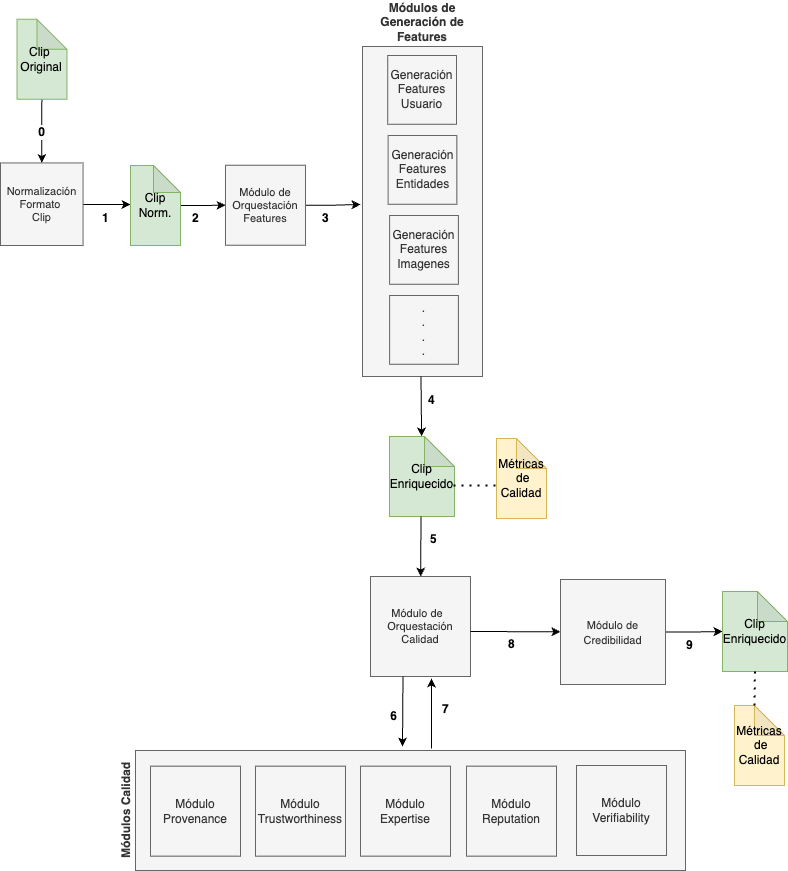
\includegraphics[width=\linewidth,height=.35\textheight,keepaspectratio]{figures/processing-flow-white}
  \caption{Flujo modular de procesamiento para evaluar credibilidad~\cite{GarciaParra2024Thesis}.}
  \Description{Flujo de procesamiento desde clip original a clip normalizado, generaci\'on de features, m\'odulos de calidad y clip enriquecido.}
  \label{fig:processing-flow}
\end{figure}

\autoref{fig:processing-flow} resume el workflow l\'ogico. El clip normalizado es el
contrato entre la ingesta espec\'ifica de cada plataforma y el c\'alculo de calidad.
Este contrato es importante porque las plataformas exponen campos, pol\'iticas y APIs
distintas. Un clip normalizado contiene contenido, URI de plataforma, metadatos del
autor, links, menciones, reacciones, comentarios, salidas de features y m\'etricas de
calidad necesarias por los m\'odulos posteriores.

La generaci\'on de features se separa del c\'alculo de m\'etricas. Un m\'odulo de feature
puede extraer una profesi\'on m\'edica desde el perfil de usuario, detectar si se
menciona una instituci\'on, calcular tama\~no de audiencia o identificar enlaces
externos. Luego, un m\'odulo de calidad mapea esas features a un valor en $[0,1]$
mediante f\'ormulas, reglas o modelos. Esta separaci\'on permite agregar extractores
sin cambiar la sem\'antica del modelo de calidad.

El m\'odulo de provenance distingue interacciones expl\'icitas e impl\'icitas. Las
expl\'icitas son mecanismos propios de las plataformas: retweets, respuestas, citas o
compartidos. Las impl\'icitas ocurren cuando los usuarios copian, parafrasean o
republican contenido sin preservar un enlace directo. Estos casos son frecuentes en
cross-sharing, donde el contenido se mueve entre plataformas y puede perder sus
metadatos originales.

\begin{figure}[t]
  \centering
  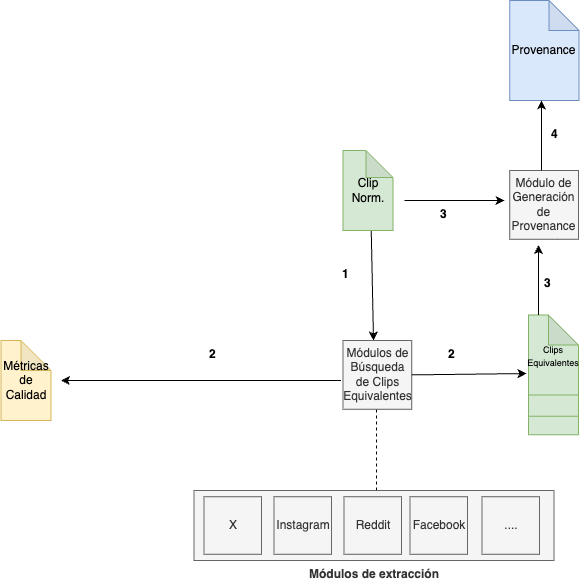
\includegraphics[width=\linewidth,height=.30\textheight,keepaspectratio]{figures/provenance-framework-white}
  \caption{Framework para buscar clips equivalentes y generar provenance~\cite{GarciaParra2024Thesis}.}
  \Description{Workflow de generaci\'on de provenance con clips normalizados, m\'odulos de b\'usqueda, clips equivalentes, m\'etricas y salida de provenance.}
  \label{fig:provenance-framework}
\end{figure}

Para abordar las interacciones impl\'icitas, el flujo usa equivalencia entre clips.
Para clips de texto, instanciamos la equivalencia mediante similitud coseno con
TF-IDF~\cite{Yuntao2005}. Dados dos clips $c_1$ y $c_2$, su similitud textual es:
\begin{equation}
  Sim(c_1,c_2) = \frac{c_1 \cdot c_2}{\|c_1\|\|c_2\|}.
\end{equation}
Los clips equivalentes se representan luego mediante una estructura inspirada en
PROV-SAID. Adaptamos PROV-SAID sustituyendo mensajes por clips, agregando el
atributo \texttt{SocialNetwork}, modelando derivaciones entre plataformas y
asociando m\'etricas de calidad a las entidades del provenance.

\autoref{fig:provenance-framework} muestra este subflujo. El m\'odulo de b\'usqueda
puede usar coincidencia exacta, fuzzy matching, b\'usqueda sem\'antica, expansi\'on de
consultas, b\'usqueda multiling\"ue o b\'usqueda contextual con hashtags, URLs, fechas
y menciones. En la prueba de concepto restringimos la equivalencia a texto, pero el
modelo admite futuras m\'etricas multimodales para im\'agenes y videos.

\subsection{Trustworthiness Path Stability}

La principal m\'etrica derivada de provenance es \emph{Trustworthiness Path
Stability}. Mide si el trustworthiness permanece estable durante la propagaci\'on.
Sea $T_i$ el valor de trustworthiness del $i$-\'esimo clip en un camino de provenance
de largo $n$. Definimos:
\begin{equation}
  TPS = 1 - \frac{\sum_{i=1}^{n-1}|T_{i+1}-T_i|}{n-1}.
\end{equation}
Valores cercanos a 1 indican estabilidad. Valores bajos indican fluctuaciones,
posiblemente causadas por modificaciones del contenido, p\'erdida de calidad de la
fuente o propagaci\'on a trav\'es de actores menos confiables.

Por ejemplo, consideremos un camino con valores de trustworthiness
$(0.90,0.85,0.88,0.86)$. La variaci\'on total entre nodos consecutivos es
$0.05+0.03+0.02=0.10$, por lo tanto $TPS=1-0.10/3=0.9667$. El valor indica que la
credibilidad no se degrad\'o materialmente durante el camino. Esto es \'util en
cross-sharing porque el mismo contenido puede preservar su claim aunque sea copiado
a un contexto social diferente.

\section{Prueba de Concepto}

Se implement\'o una prueba de concepto para clips de salud relacionados con
estatinas y colesterol. El dominio fue elegido porque la desinformaci\'on sobre
estatinas puede influir en la adherencia a tratamientos y en decisiones de salud
p\'ublica. La implementaci\'on se despleg\'o en Google Cloud Platform con Pub/Sub
para ingesta, Cloud Storage para persistencia, Cloud Functions para m\'odulos de
features y calidad, y Cloud Composer para orquestaci\'on.

El experimento parti\'o de 97 clips recolectados en varias plataformas mediante
keywords sobre estatinas y colesterol. Se preseleccionaron once clips para cubrir
distintas redes y niveles de credibilidad. Un experto m\'edico clasific\'o los clips y
asign\'o puntajes.

Para el experimento, trustworthiness se calcul\'o con tres m\'etricas: access to source
data, certification y confidence. El experto asign\'o ponderadores de 0.4, 0.4 y 0.2,
respectivamente. Credibility combin\'o Trustworthiness Path Stability y
trustworthiness con ponderadores de 0.6 y 0.4 cuando hab\'ia provenance disponible.
Cuando no hab\'ia provenance, el modelo se apoy\'o solo en trustworthiness.

Los m\'odulos de features implementados se enfocaron en evidencia de perfiles
m\'edicos. Extrajeron profesi\'on m\'edica, educaci\'on m\'edica, verificabilidad m\'edica
e influencia m\'edica a partir de informaci\'on p\'ublica de perfiles y evidencia
textual disponible. Luego, los m\'odulos de calidad calcularon certification, access
to source data, confidence, trustworthiness, Trustworthiness Path Stability y
credibilidad final. Los umbrales fueron conservadores: 0.00 a 0.50 para baja
credibilidad, 0.51 a 0.75 para media y 0.76 a 1.00 para alta.

\begin{table}[t]
  \caption{Comparaci\'on entre juicio experto y salida del modelo~\cite{GarciaParra2024Thesis}.}
  \label{tab:results}
  \begin{tabular}{ccccc}
    \toprule
    Clip & Experto & Score & Modelo & Cred.\\
    \midrule
    1 & Medio & 0.60 & Alto & 0.80\\
    2 & Medio & 0.70 & Medio & 0.68\\
    3 & Medio & 0.60 & Medio & 0.68\\
    4 & Medio & 0.70 & Medio & 0.64\\
    5 & Medio & 0.60 & Alto & 0.78\\
    6 & Bajo & 0.00 & Bajo & 0.09\\
    7 & Bajo & 0.00 & Bajo & 0.18\\
    8 & Bajo & 0.00 & Bajo & 0.11\\
    9 & Bajo & 0.10 & Bajo & 0.09\\
    10 & Bajo & 0.00 & Bajo & 0.08\\
    11 & Bajo & 0.00 & Bajo & 0.36\\
    \bottomrule
  \end{tabular}
\end{table}

El modelo coincidi\'o con el nivel experto en nueve de los once clips
(\autoref{tab:results}). Las dos diferencias corresponden a clips donde el
provenance aument\'o la credibilidad: ambos ten\'ian caminos estables y hab\'ian sido
compartidos por usuarios con trustworthiness relativamente alto. El experto no
ten\'ia acceso a todos los perfiles involucrados en la propagaci\'on, por lo que su
puntaje se acerc\'o m\'as al trustworthiness aislado que al valor final sensible al
provenance.

La implementaci\'on preliminar obtuvo un tiempo promedio de ejecuci\'on de 5220 ms
por clip. Aunque el resultado es alentador, la muestra es peque\~na para realizar
afirmaciones sobre escalabilidad o precisi\'on predictiva. El valor del experimento
es mostrar que un modelo de calidad puede producir m\'etricas interpretables y
exponer cu\'ando el provenance cambia la evaluaci\'on.

Las m\'etricas detalladas tambi\'en explican los resultados. Los clips publicados por
cuentas con credenciales m\'edicas expl\'icitas y referencias institucionales
verificables obtuvieron mayores valores en certification y access to source data.
Los clips provenientes de perfiles autoproclamados o pseudocient\'ificos obtuvieron
baja expertise incluso cuando ten\'ian se\~nales de audiencia. Confidence tuvo menor
peso para evitar sobrevalorar popularidad en un dominio m\'edico sensible.

\section{Discusi\'on}

El modelo propuesto desplaza la medici\'on de credibilidad desde una predicci\'on
monol\'itica hacia un flujo de calidad de datos. Esto tiene dos ventajas para QDB.
Primero, explicita los criterios: se puede inspeccionar si el score proviene de
verificabilidad, expertise, reputation o estabilidad del provenance. Segundo, separa
conocimiento de dominio e infraestructura. En medicina se puede usar certification
y access to source data, mientras que otros dominios pueden definir otras features y
umbrales.

Existen limitaciones. La prueba de concepto usa pocos clips y un \'unico experto de
dominio. La estrategia de equivalencia cubre solo texto y no incluye im\'agenes o
video. La reconstrucci\'on de provenance depende de APIs, buscadores y metadatos
p\'ublicos disponibles. Finalmente, el modelo asume que los expertos pueden definir
ponderadores significativos; trabajos futuros deber\'ian comparar calibraci\'on
manual, basada en reglas y aprendida.

\subsection{Trabajo Futuro}

Como trabajo futuro se propone ampliar la evaluaci\'on a datasets mayores, m\'as
plataformas y m\'ultiples expertos de dominio, para medir acuerdo entre evaluadores
y transferibilidad entre dominios. Una segunda l\'inea es la equivalencia multimodal
entre clips, incluyendo im\'agenes, video, capturas de pantalla y par\'afrasis
parciales, ya que el contenido enga\~noso suele propagarse mediante cambios de
formato y no solo por reutilizaci\'on textual exacta. Esto tambi\'en motiva el uso
de modelos peque\~nos de lenguaje (SLM) para procesar clips desde im\'agenes, como
capturas de pantalla o publicaciones renderizadas, dado que el acceso a las APIs
de redes sociales es cada vez m\'as restringido y heterog\'eneo entre plataformas.
Estos SLM deber\'ian ejecutarse en el edge, sin enviar clips a la nube, para
preservar la privacidad; adem\'as, el modelo de calidad de credibilidad deber\'ia
integrarse al pipeline del SLM, de modo que la evidencia visual y textual extra\'ida
se mapee directamente a dimensiones y m\'etricas de calidad.
El componente de provenance tambi\'en deber\'ia incorporar metadatos de calidad sobre completitud, confianza,
incertidumbre y enlaces faltantes. Finalmente, se requiere avanzar en la
calibraci\'on de pesos y en visualizaciones para usuarios finales que expliquen c\'omo
cada dimensi\'on de calidad contribuye al score final de credibilidad.

\section{Conclusi\'on}

Este paper present\'o un modelo de calidad de datos, sensible al provenance, para
medir credibilidad en plataformas de redes sociales. Al combinar trustworthiness,
provenance, equivalencia entre clips y Trustworthiness Path Stability, el modelo
ofrece una forma interpretable de evaluar contenido social entre plataformas y
dominios. La prueba de concepto sobre estatinas sugiere que el provenance puede
cambiar materialmente la evaluaci\'on de credibilidad y debe tratarse como una
se\~nal de calidad de primer orden.

\begin{acks}
TODO: Agregar financiamiento, tutor\'ia, agradecimientos institucionales y
agradecimientos al experto de dominio seg\'un corresponda.
\end{acks}

\bibliographystyle{ACM-Reference-Format}
\bibliography{references}

\end{document}
\endinput
